\newcommand\UniversiteAdi{Niğde Ömer Halisdemir Üniversitesi}
\newcommand\BolumAdi{MEKATRONİK BÖLÜMÜ}
\newcommand\DersKodu{MKT2002}
\newcommand\DersAdi{BİLGİSAYARLI KONTROL SİSTEMLERİ}
\newcommand\SinavAdi{Ödev 2}
\newcommand\SinavTarihi{10.03.2025}
\newcommand\SinavSaati{10:00}
\newcommand\SinavSuresi{90dk}

\pagestyle{fancy}
\fancyhf{} % clear existing header/footer entries
\fancyhead[R]{Öğrenci No:\hspace{4.5cm}}
\fancyhead[L]{Ad Soyad:\hspace{7cm}}
\noindent
\begin{tabular}{
    p{0.15\linewidth}
    p{0.15\linewidth}
    p{0.3\linewidth}
    p{0.1\linewidth}
    p{0.15\linewidth}}
    \multicolumn{5}{c}{\textbf{\BolumAdi}}\\
    \multicolumn{5}{c}{\textbf{\DersAdi}}\\\hline
    \multicolumn{1}{|r|}{Ders Kodu:}&
    \multicolumn{1}{|c|}{\DersKodu}&
    \multicolumn{1}{|c|}{}& 
    \multicolumn{1}{|r|}{Tarih:}&
    \multicolumn{1}{|c|}{\SinavTarihi} \\\hline
    \multicolumn{1}{|r|}{Sınav Türü:}&
    \multicolumn{1}{|c|}{\SinavAdi}&  
    \multicolumn{1}{|c|}{}&
    \multicolumn{1}{|r|}{Saat:}&
    \multicolumn{1}{|c|}{\SinavSaati}\\\hline
    \multicolumn{1}{|r|}{Dönemi:}&
    \multicolumn{1}{|c|}{2024-2025}&
    \multicolumn{1}{|c|}{}&
    \multicolumn{1}{|r|}{Süre:}&
    \multicolumn{1}{|c|}{\SinavSuresi} \\\hline
    &&&&\\
\end{tabular}\\\\
\noindent\begin{center}
\begin{tabular}{|r|c|}\hline
    &\textbf{Toplam}\\\hline
    \textbf{Puan:} &\textbf{100}\\\hline
    \textbf{Not:}  &110\\\hline
\end{tabular}\end{center}
\noindent\textbf{Uyarı:}
\begin{itemize}\bfseries
    \item Soruları dikkatlice okuyunuz. Hesap makinesi kullanılabilir.
    \item İşlemleri atlamadan ve ayrıntılı olarak veriniz. Sadece nümerik yanıtlar veya çizimler ara işlemler olmadan kabul edilmemektedir.
\end{itemize}
\noindent\textbf{Soru:} Bir sistem transfer fonksiyonu 
\begin{equation}
    G(s)=\frac{1}{s^2+2s+4}
\end{equation}
olarak verilmiştir. Bir kutup eklenmesi durumunda 
\begin{equation}
    G_1(s)=G(s)\frac{p}{s+p}
\end{equation}
veya bir sıfır eklenmesi durumunda 
\begin{equation}
    G_2(s)=G(s)\frac{s+z}{z}
\end{equation}
oluşan sistemin basamak yanıtını inceleyiniz. Bunun için eklenen kutup veya sıfırı iki farklı aralıkta $0.1\leq z,p\leq 0.5$ ve $5\leq z,p\leq10$ inceleyiniz. Kutupların incelemesi için Şekil~\ref{fig:plot1} ve Şekil~\ref{fig:plot2} ile verilmiştir. 

\begin{figure}[!htb]
    \centering
    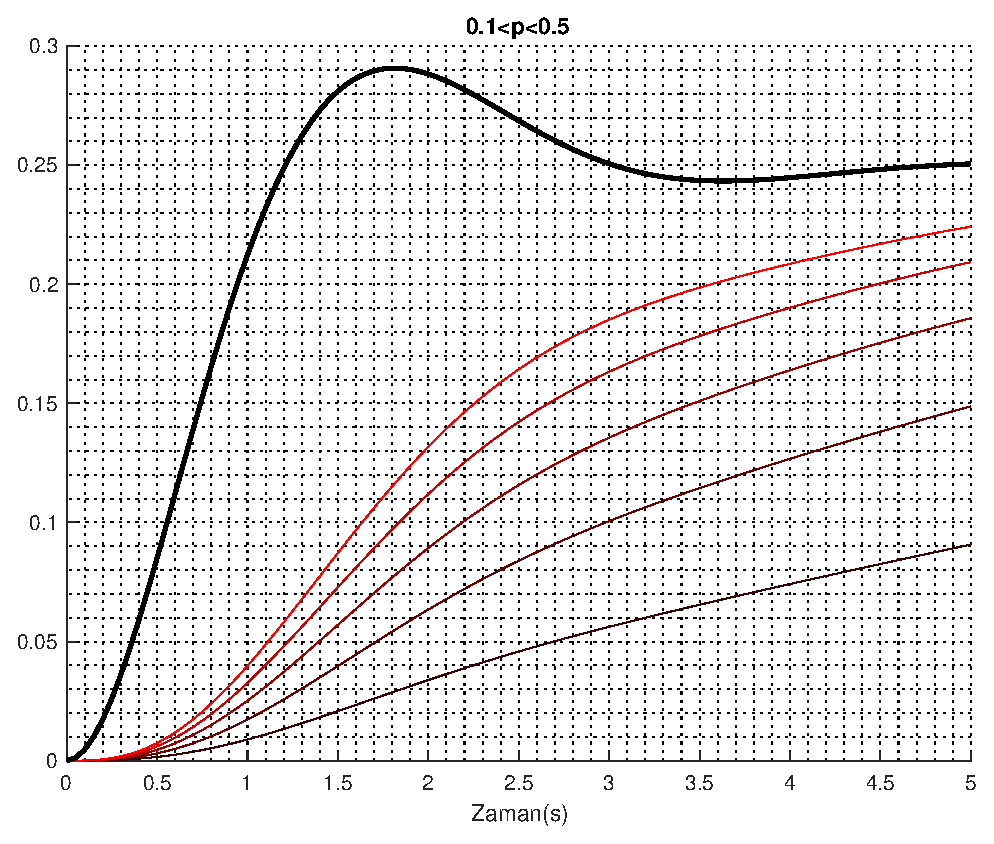
\includegraphics[width=0.5\textwidth]{plot1}
    \caption{$0.1\leq p\leq 0.5$ için basamak yanıtlarının değişimi}\label{fig:plot1}
\end{figure}

\begin{figure}[!htb]
    \centering
    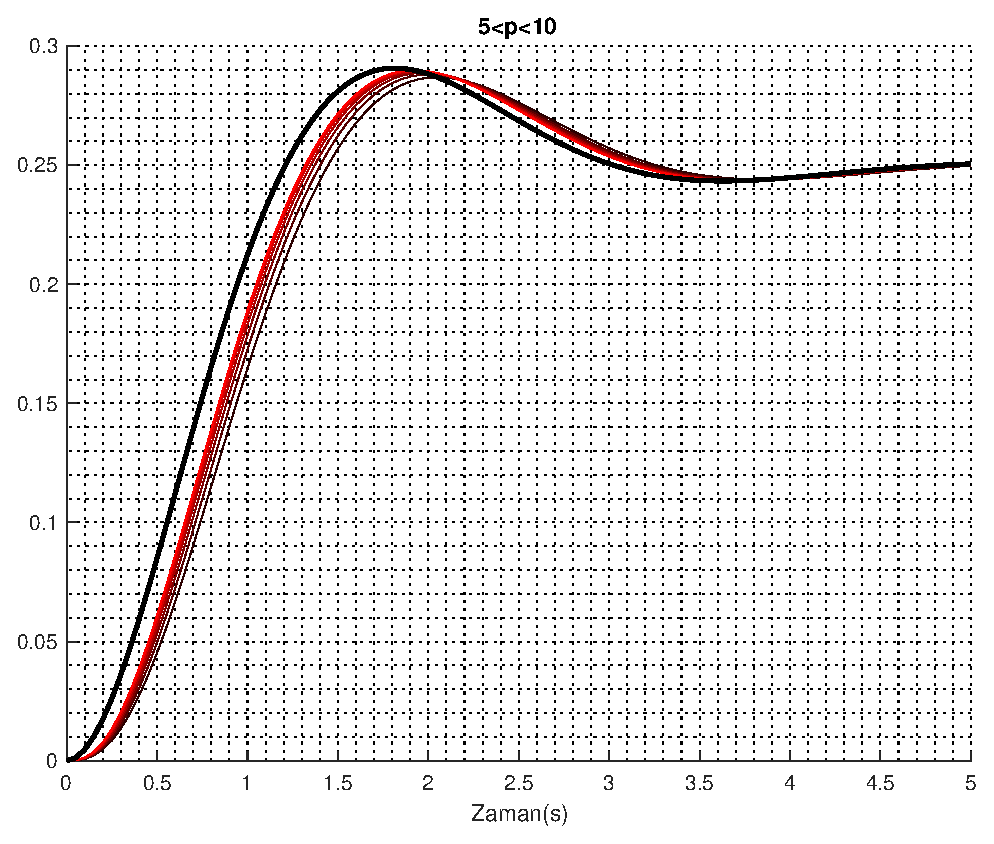
\includegraphics[width=0.5\textwidth]{plot2}
    \caption{$1\leq p\leq 5$ için basamak yanıtlarının değişimi}\label{fig:plot2}
\end{figure}

Grafikleriden görüldüğü üzere, baskın bölgenin dışına eklenen bir kutup basamak yanıtını isterler açısından çok etkilememektedir. Baskın bölgede eklenmesi ise isterleri bozmaktadır.

Sıfırların incelemesi için Şekil~\ref{fig:plot3} ve Şekil~\ref{fig:plot4} ile verilmiştir. 

\begin{figure}[!htb]
    \centering
    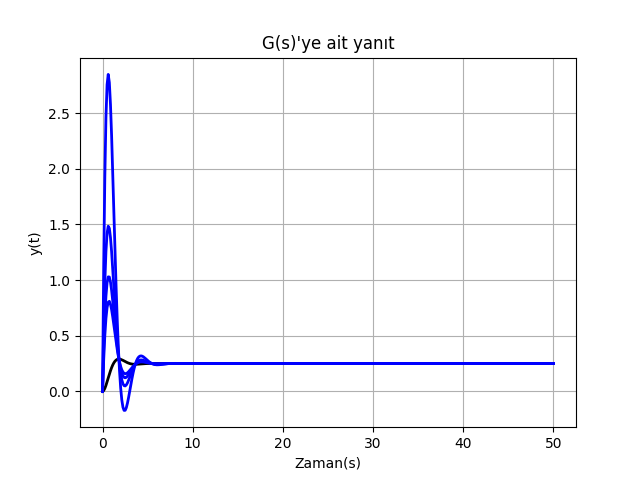
\includegraphics[width=0.5\textwidth]{plot3}
    \caption{$0.1\leq z\leq 0.5$ için basamak yanıtlarının değişimi}\label{fig:plot3}
\end{figure}

\begin{figure}[!htb]
    \centering
    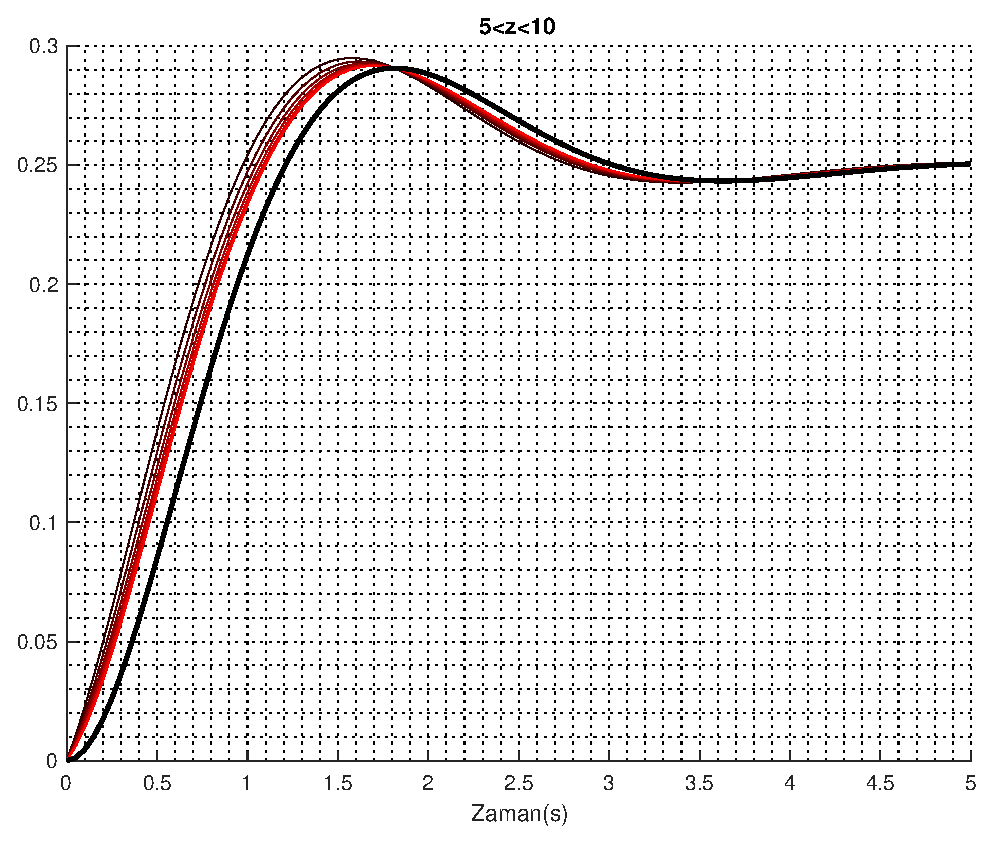
\includegraphics[width=0.5\textwidth]{plot4}
    \caption{$1\leq z\leq 5$ için basamak yanıtlarının değişimi}\label{fig:plot4}
\end{figure}

Grafikleriden görüldüğü üzere, baskın bölgenin dışına eklenen bir sıfır basamak yanıtını isterler açısından çok etkilememektedir. Baskın bölgede eklenmesi ise isterleri bozmaktadır ve kutup eklemekten daha çok bozulma meydana gelmektedir.